\chapter{Implementation}
Nun da die Grundlagen gelegt sind können wir anfangen zu untersuchen wie ein LSTM Netz mit Events umgeht. Wir betrachten dazu das Bouncing Ball Szenario, da es klare Events hat und sich dadurch auch gut segmentieren lässt. Zur Implementation wurde JANNLab (Otte et al. 2013), ein Java Framework für Neuronale Netze verwendet \ref{bib:jannlab}. Dieses Kapitel soll die im Zuge dieser Arbeit verwendeten Techniken erklären und aufzeigen wie die im nächsten Kapitel beschriebenen Ergebnisse erreicht wurden, sowie welche Probleme sich dabei in den Weg gestellt haben.

\section{Das Bouncing Ball Szenario}
Das Bouncing Ball Szenario beschreibt einen Ball, der zwischen Begrenzungen umher gleitet und an diesen abprallt. Wir haben die 1- und die 2-dimensionale Version verwendet.

Im 1-D Fall haben wir einen Ball ohne Ausdehnung (also eigentlich ein Punkt aber diese Unterscheidung ist für unsere Zwecke irrelevant) mit einer Position $ x_{b} $ und einer konstanten Geschwindigkeit $  v$. Dieser springt zwischen den Grenzen $ x_{1}=-1 $ und $ x_{2}=1 $ hin und her, also immer wenn die Position des Balls eine der Grenzen annimmt, wird die Geschwindigkeit invertiert $ v := -v $. Also genau so wie man es sich vorstellt.

Der 2D Fall funktioniert analog, der Ball hat eine Position $ (x_{b}/y_{b}) $, eine konstante Geschwindigkeit $ (v_{x}/v_{y}) $, welcher nun zwischen den 4 Grenzen $ x_{1}=-1 $ und $ x_{2}=1 $, $ y_{1}=-1 $ und $ y_{2}=1 $ hin und her springt. Nimmt nun eine Koordinate des Balls eine der Grenzen an wird die entsprechende Koordinate invertiert, also $ (v_{x}/v_{y}) = (-v_{x}/v_{y}) $ beziehungsweise $ (v_{x}/-v_{y}) $. 

Das 1D-Szenario habe ich hauptsächlich verwendet um mich einzuarbeiten und zurechtzufinden, da es unter anderem mit weniger Neuronen erlernt werden kann und so die Aktivierungen der einzelnen Gates auch übersichtlicher sind. Der Grund warum das 1D-Szenario auch für diese Ausarbeitung wichtig ist, ist das unter Hinzunahme der Zeitachse aussagekräftige Diagramme erstellt werden können, anhand derer einige Trainingseffekte und Verläufe veranschaulicht werden können. Entsprechende Analysen konnten vom 2D-Fall auch gemacht werden, wenn man sah wie sich eine Linie oder ein Ball mit Verzögerung entsprechend über den Bildschirm bewegt, die resultierenden Bilder sind jedoch eher unübersichtlich. Das 2D Szenario hingegen ist das für unsere Untersuchungen interessantere, da es mehr Events gibt, die auch in komplexernen Beziehungen zueinander stehen.
\begin{figure}
	\centering
	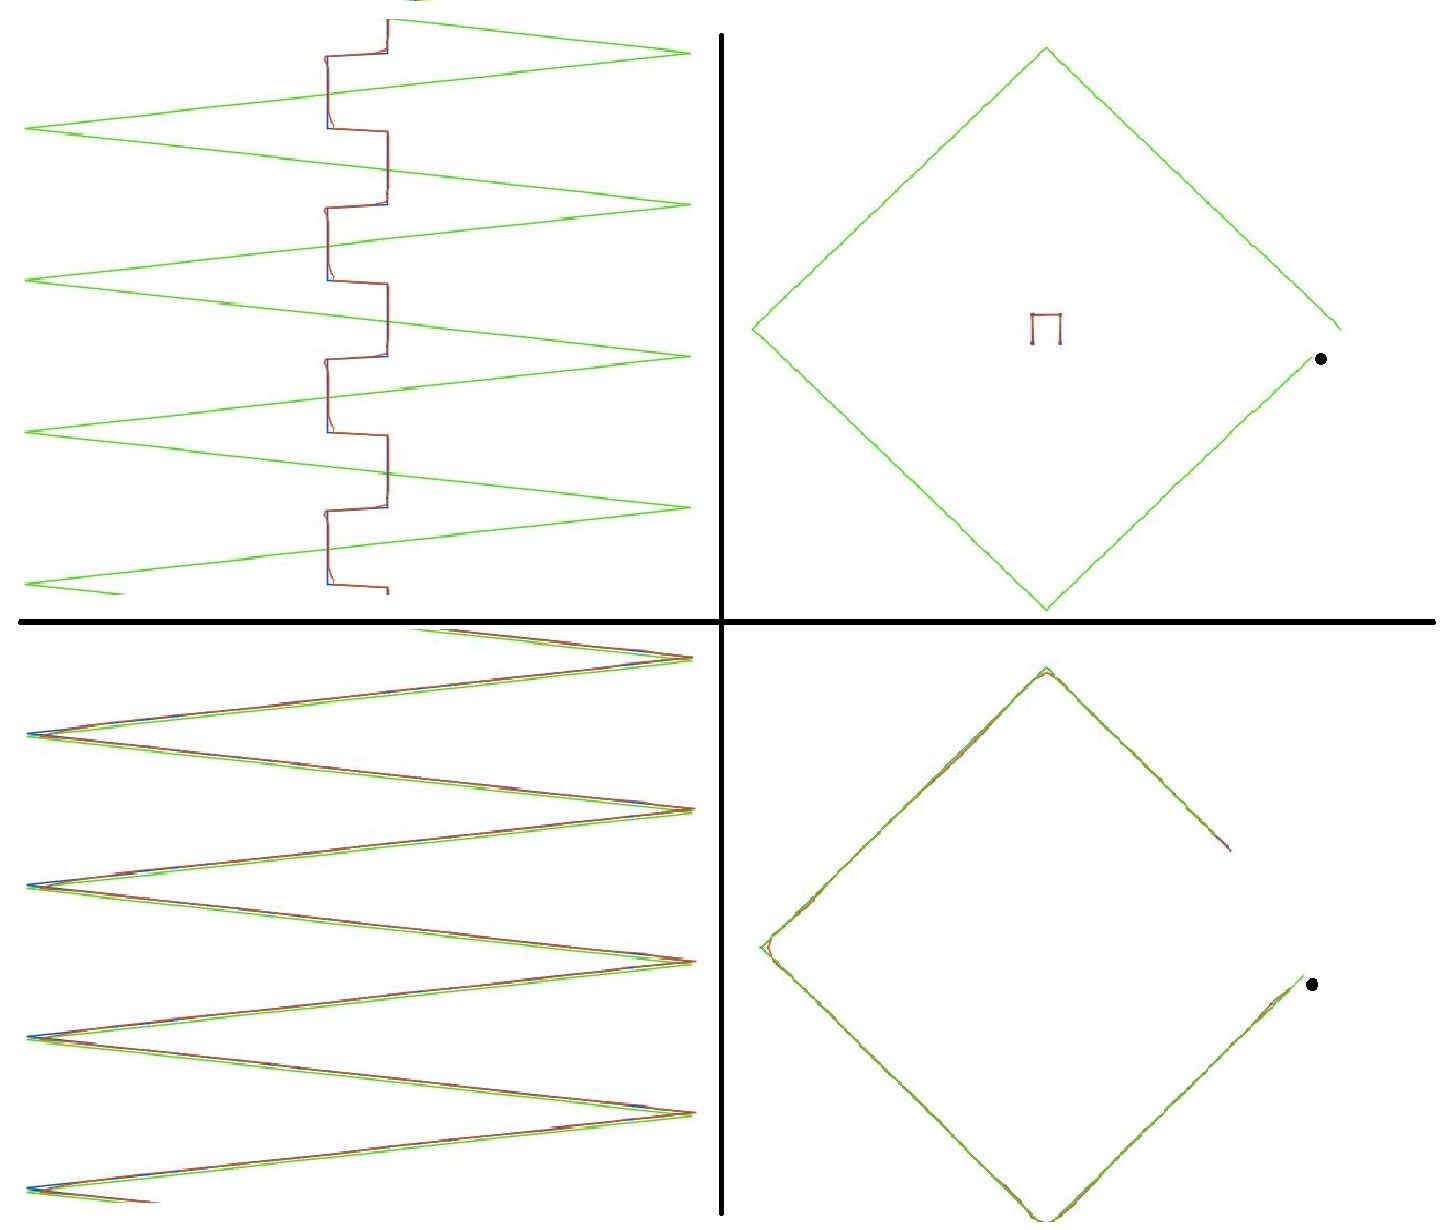
\includegraphics[width=0.9\textwidth, height=350px]{pics/1dvs2d.jpg}	
	\caption{Schematische Darstellung einer Möglichkeit, ein künstliches Neuron zu simulieren}
	\label{img:aneuron}
\end{figure}

\section{Unser LSTM, Parameter + Testfälle}
linearen output, da sigmoid 0-1


\section{Das Training des Bouncing Verhaltens}




\section{Feedback}

Das 1D Szenario habe ich hauptsächlich verwendet um mich einzuarbeiten und zurechtzufinden, da es unter anderem mit weniger Neuronen erlernt werden kann und so die Aktivierungen der einzelnen Gates auch übersichtlicher sind. Der Hauptvorteil und warum das 1D Szenario auch für diese Ausarbeitung wichtig ist, das unter hinzunahme der Zeitachse aussagekräftige Diagramme erstellt werden können, anhand derer einige Trainingseffekte und Verläufe veranschaulicht werden können. Entsprechende Analysen konnten vom 2D Fall auch gemacht werden, wenn man sah wie sich eine Linie  oder ein Ball mit Verzögerung entsprechend über den Bildschirm bewegt, die resultierenden Bilder sind jedoch eher unübersichtlich. Das 2D Szenario hingegen ist das für unsere Untersuchungen interessantere, da es mehr Events gibt, die auch in komplexernen Beziehungen zueinander stehen, hierzu mehr in Kaptel 3.999.

Das Training des Bouncing Verhaltens
Das interessante am Bouncing Ball Szenario ist natürlich nicht die gleichförmige Bewegung, sondern das nicht-lineare Verhalten beim Abprallen. Dieses wollen wir unserem LSTM Netzwerk möglichst genau erlernen und haben dazu einige Techniken angewendet. 

Reaktives vs vorhersehendes Verhalten
1D mit 1b Zelle

RNN Annäherung vs echte nichtlinearität
Random vs nicht Random, nur periodisch gelernt
Feedback für random, erklären warum es nicht funkltioniert hat,
Feedback, Zittern erklären für Input außerhalb des eigenen Raums
Schritte damit es funktioniert, feedback annäherung, hat nicht geholfen
Random diskretisiert um numerisch genau definiertes Rand verhalten zu haben